\documentclass[aspectratio=1610,pdftex,dvipsnames]{beamer}
\usetheme{Boadilla}
\usecolortheme{seahorse}
\beamertemplatenavigationsymbolsempty 
\addtobeamertemplate{footnote}{\hskip -2em}{}

\definecolor{BackGround}{RGB}{255,250,240}
\setbeamercolor{background canvas}{bg=BackGround}

\usepackage{caption}
\captionsetup[figure]{labelformat=empty}

%packages and definitions
\usepackage{enumitem}
\setlist[itemize]{label=\textbullet}
\usepackage{amsmath,cancel,nicefrac}
\usepackage{ulem}
\usepackage{graphicx,animate}
%\usepackage{mypythonhighlight}% allows inclusion of graphics
\graphicspath{{../img/}} %path to graphics
\usepackage[yyyymmdd]{datetime} %date format
\renewcommand{\dateseparator}{.}

%%%%%
\usepackage{pgf}
\usepackage{tikz} % required for drawing custom shapes
\usetikzlibrary{shapes,arrows,automata,trees}
%%%%%

\usepackage{booktabs} % nice rules (thick lines) for tables
\usepackage{microtype} % improves typography for PDF

\usepackage[acronym,nomain,nonumberlist]{glossaries}
%\makenoidxglossaries

\usepackage{xcolor,colortbl} %change font color
\usepackage[numbers,sort&compress]{natbib} %use 'numbers' for numbered citations; 'round' for () instead [] for inline citations; nsf.bst
\usepackage{bibentry}


\setlength{\bibsep}{0pt} %sets space between references
%\renewcommand{\bibsection}{} %suppresses large 'references' heading
\renewcommand\bibpreamble{\vspace{-0.2\baselineskip}} %sets spacing after heading if not using default references heading

%%%%% user commands
\newcommand\blfootnote[1]{%
  \begingroup
  \renewcommand\thefootnote{}\footnote{#1}%
  \addtocounter{footnote}{-1}%
  \endgroup
}


\makeatletter
\renewcommand{\@biblabel}[1]{#1.\hfill} %bibliography ordered list has numbers left flush
\makeatother

\newcommand{\edit}[1]{\textcolor{blue}{#1}} %shortcut for changing font color on revised text
\newcommand{\fn}[1]{\footnote{#1}} %shortcut for footnote tag
\newcommand*\sq{\mathbin{\vcenter{\hbox{\rule{.3ex}{.3ex}}}}} %makes a small square as a separator $\sq$
\newcommand{\sk}[1]{\sout{#1}} %shortcut for strikethrough
\newcommand{\x}{\cellcolor{lightgray}} %use to shade in table cell

\newcommand{\acf}{\acrfull} %full acronym
\newcommand{\acl}{\acrlong} %long acronym
\newcommand{\acs}{\acrshort} %short acronym
\newcommand{\acfp}{\acrfullpl} %full acronym plural
\newcommand{\aclp}{\acrlongpl} %long acronym plural
\newcommand{\acsp}{\acrshortpl} %short acronym plural
\newcommand{\Acf}{\Acrfull} %full acronym first letter capital
\newcommand{\Acl}{\Acrlong} %long acronym first letter capital

\newacronym{pid}{PID}{Proportional-Integral-Derivative}
\newacronym{msnb}{MSNB}{Molten Salt Nuclear Battery}

%%%%%

%%%%%



\title[\acs{pid} Controller Design: \acs{msnb}]{Design of a \acs{pid} Controller for a Molten Salt Microreactor}
\subtitle{Master's Plan}
\author[Root]{Sam J. Root,\textsuperscript{1}\\
    Major Professor: Michael McKellar,\textsuperscript{1}\\
    Committee Members: Robert A. Borrelli\textsuperscript{1}, 
    Dakota Roberson\textsuperscript{2}
    }
\institute[Idaho Falls Center]{\vspace{0.5cm}\\
    University of Idaho $\sq$ Idaho Falls Center for Higher Education\\
    \textsuperscript{1}Department of Nuclear Engineering and Industrial Management\\
    \textsuperscript{2}Department of Electrical and Computer Engineering\\
    \vspace{0.10in}
    %
\includegraphics[width=0.20\textwidth]{ne-logo.jpg}
    }

\date{2022.10.13}
    
\begin{document}


\nobibliography*


{    \setbeamertemplate{footline}{} 
    \begin{frame}
        \titlepage
    \end{frame}
} 

\begin{frame}{Xenon-135 Decay Chain}
    \only<1>{
    \begin{itemize} 
        \item Xenon-135 has a neutron capture cross-section of more than $2Mb$;
        \item Iodine-135 is a common products of Uranium-235 fission;
        \item $^{135}Xe$ is formed by $^{135}I$ $\beta$-decay ($t_{\nicefrac{1}{2}}\approx 7 \; hrs$);
    \end{itemize}}
    \vspace{1cm}

    \only<2>{

    \begin{table}[h!]
    \caption{Relevant nuclear constants \cite[Ch. 7]{Lamarsh}}
    \centering\begin{tabular}{c|cccc}
     & $\gamma \;(\%)$ & $\lambda \; (hr^{-1})$ & $t^{\nicefrac{1}{2}} (hr)$ & $\sigma \; (Mb)$ \\ \hline
     $^{135}I$ & 6.39 & 0.1035 & 6.57 & - \\
     $^{135}Xe$ & 0.237 & 0.0753 & 9.14 & 2.65
    \end{tabular}
    \label{params}
    \end{table}}


    
    \blfootnote{\tiny\cite{Lamarsh}\tiny\bibentry{Lamarsh}}
    
    \begin{equation*}\label{diffI}
        \frac{dI}{dt} =
        \underbrace{\gamma_{I}\Sigma_{f}^{F}{\phi}(t)}_{\text{Fission Yield}}
        -\underbrace{\lambda_{I}I(t)}_{\text{Beta Decay}}
    \end{equation*}
    \begin{equation*}\label{diffXe}
        \frac{dXe}{dt} =
        \underbrace{\gamma_{Xe}\Sigma_{f}^{F}{\phi}(t)}_{\text{Fission Yield}}
        +\underbrace{\lambda_{I}I(t)}_{\text{Precursor Decay}}
        -\underbrace{\lambda_{Xe}Xe(t)}_{\text{Beta Decay}}
        -\underbrace{Xe(t)\sigma_{a}^{Xe}{\phi}(t)}_{\text{Radiative Capture}}
    \end{equation*}

\end{frame}

\begin{frame}{Numerical Solver (Euler's Method)}
    \begin{equation*}
        I[t+dt]=I[t]+\frac{dI}{dt}[t]
    \end{equation*}
    \begin{equation*}
        Xe[t+dt]=Xe[t]+\frac{dXe}{dt}[t]
    \end{equation*}

    \only<2>{\vspace{1cm}\begin{itemize}
        \item 1 second time steps;
        \item Able to change neutron flux (i.e. scram) at any time step;
        \item Tracks absolute concentration as well as the contribution to the overall rate of change by each term in the differential equations vs. time;
    \end{itemize}}
\end{frame}

\begin{frame}{Xenon-135 Decay Chain: Start-up}
    \begin{columns}
    %Column 1
    \begin{column}{0.5\textwidth}
    \only<1> {
    \begin{figure}
        %\animategraphics[width=0.99\textwidth, controls]{2}{../img/equilibrium/bar-}{1}{48}
        \caption{Nuclide Concentration Rates of Change - Reactor Start-up}
    \end{figure}
    }

    \only<2> {
    \addtocounter{figure}{1}
   
    \begin{equation*}
        I_{\infty}(\phi) = \frac{\gamma_I \Sigma_f^F }{\lambda_I}\phi
    \end{equation*}
    \begin{equation*}
        Xe_{\infty}(\phi) = \frac{(\gamma_I+\gamma_{Xe}) \Sigma_f^F }{\lambda_I+\sigma_a^{Xe}\phi}\phi
    \end{equation*}
    }
    \end{column}
    %Column 2
    \begin{column}{0.5\textwidth}
    \begin{figure}
        %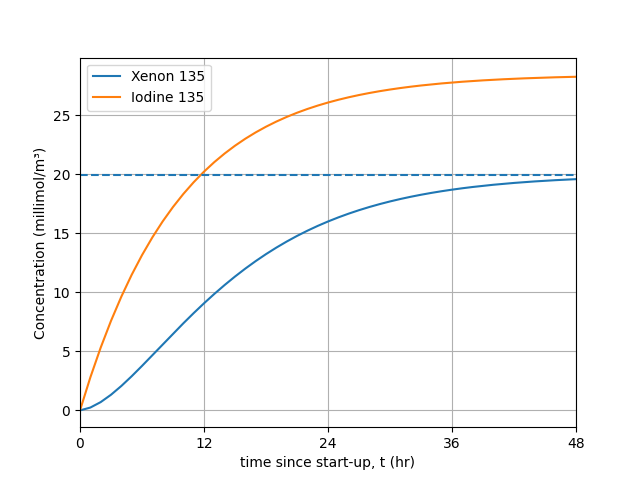
\includegraphics[width=0.99\textwidth]{start-up}
        \caption{Nuclide Concentration - Reactor Start-up}
    \end{figure}

    \end{column}
    \end{columns}
    \only<2>{\blfootnote{\tiny\cite{Lamarsh}\tiny\bibentry{Lamarsh}}}
\end{frame}

\begin{frame}{Xenon-135 Decay Chain: Scram}
    \only<1>{
    \begin{equation*}
    \frac{dI}{dt} =
    \cancelto{0}{\underbrace{\gamma_{I}\Sigma_{f}^{F}{\phi}(t)}_{\text{Fission Yield}}}
    -\underbrace{\lambda_{I}I(t)}_{\text{Beta Decay}}
    \end{equation*}
    \begin{equation*}
    \frac{dXe}{dt} =
    \cancelto{0}{\underbrace{\gamma_{Xe}\Sigma_{f}^{F}{\phi}(t)}_{\text{Fission Yield}}}
    +\underbrace{\lambda_{I}I(t)}_{\text{Precursor Decay}}
    -\underbrace{\lambda_{Xe}Xe(t)}_{\text{Beta Decay}}
    -\cancelto{0}{\underbrace{Xe(t)\sigma_{a}^{Xe}{\phi}(t)}_{\text{Radiative Capture}}}
    \end{equation*} 
    }

    \only<2>{
    \begin{equation*}
    \frac{dI}{dt} =
    -\underbrace{\lambda_{I}I(t)}_{\text{Beta Decay}}
    \end{equation*}
    \begin{equation*}
    \frac{dXe}{dt} =
    \underbrace{\lambda_{I}I(t)}_{\text{Precursor Decay}}
    -\underbrace{\lambda_{Xe}Xe(t)}_{\text{Beta Decay}}
    \end{equation*} 
    }

    \begin{columns}
        %Column 1
        \begin{column}{0.5\textwidth}

        \only<3>{\begin{figure}
            %\animategraphics[width=0.99\textwidth, controls]{2}{../img/scram/bar-}{200}{248}
            \caption{Nuclide Concentration Rates of Change - Reactor Scram}
        \end{figure}}

        \only<4>{   \addtocounter{figure}{1} 
            \centering Bateman Equations \cite{Bateman}
            \begin{align*}
                I(t) &= I_0e^{-\lambda_I t}\\
            \begin{split}
                Xe(t) &= Xe_0e^{-\lambda_{Xe} t}\\&+\frac{\lambda_I I_0}{\lambda_I - \lambda_{Xe}}(e^{\lambda_{Xe}t}-e^{\lambda_{I}t})
            \end{split}\end{align*}
        }
        \only<5>{
            \begin{itemize}
                \item Restarting may be impossible during peak if reactor does not have enough excess control reactivity;
                \item Burn-off during premature restart is akin to positive reactivity insertion \cite{Roberson}
            \end{itemize}
        }

        \end{column}
        %Column 2
        \begin{column}{0.5\textwidth}
        \only<3->{\begin{figure}
            %%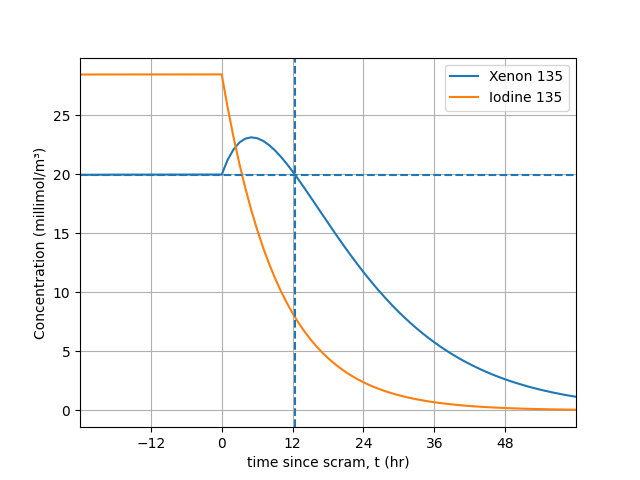
\includegraphics[width=0.99\textwidth]{../img/noHe}
            \caption{Nuclide Concentration - Reactor Scram}
        \end{figure}}

        \end{column}
    \end{columns}
    \only<4>{\blfootnote{\tiny\cite{Bateman}\tiny\bibentry{Bateman}}}
    \only<5>{\blfootnote{\tiny\cite{Roberson}\tiny\bibentry{Roberson}}}
\end{frame}

\begin{frame}{Molten Salt Reactor}
    \begin{figure}[h]\centering
    %\resizebox{0.42\textwidth}{!}{%\input{tikz_bfd}}
    \caption{Molten Salt Microreactor with Xenon Stripping Module}
    \label{BFD}
    \end{figure}

   \blfootnote{\tiny\cite{CarterPHD}\tiny\bibentry{CarterPHD}}
   \blfootnote{\tiny\cite{Peterson}\tiny\bibentry{Peterson}}
   \blfootnote{\tiny\cite{ORNL-masstransport}\tiny\bibentry{ORNL-masstransport}}
\end{frame}

\begin{frame}{Henry's Law}
    \only<1>{
    \begin{itemize}
        \item Applies to dissolved gasses at low concentration
        \item Temperature dependent relationship between the concentration of the solute in the liquid phase and the partial pressure of the solute in the cover gas.
    \end{itemize}

    \begin{equation*}
        c = Hp
    \end{equation*}}

    \only<2>{By considering total pressure of the cover gas and assuming an equation of state, Henry's law can be modified to be expressed in terms of gas phase concentration instead of partial pressure.

    \begin{equation*}
        c_{\ell} = H^{*}c_g
    \end{equation*}}

    \blfootnote{\tiny\cite{ORNL-solubility}\tiny\bibentry{ORNL-solubility}}
\end{frame}

\begin{frame}{Xenon Stripping Module}
    \begin{columns}[T]
    \begin{column}{0.5\textwidth}
    \begin{figure}[h!]\centering
    %\input{tikz_stripper}
    \caption{Schematic Drawing of Xenon Stripping Module} \label{strip}
    \end{figure}\end{column}
    \begin{column}{0.5\textwidth}

    \onslide<2->{
    \begin{equation*}
        C_{salt}^{out}=C_{salt}^{in}\left( 1+\frac{1}{H^*}\frac{\dot{V}_{He}}{\dot{V}_{salt}}  \right)^{-1}
    \end{equation*}
    }

    \onslide<3>{
    \begin{equation*}\begin{split}
    \frac{dC_{salt}}{dt} &=
    C_{He}^{out}\frac{\dot{V}_{He}}{\dot{V}_{salt}}
    =\frac{C_{salt}^{out}}{H^*}\frac{\dot{V}_{He}}{\dot{V}_{salt}}\\
    &= C_{salt}^{in}\left( H^*\frac{\dot{V}_{salt}}{\dot{V}_{He}}+1 \right)^{-1}
    \end{split}\end{equation*}
    }\end{column}\end{columns}
\end{frame}

\begin{frame}{Xenon-135 Decay Chain: With Stripping}
    \begin{equation*}\label{diffI}
        \frac{dI}{dt} =
        \underbrace{\gamma_{I}\Sigma_{f}^{F}{\phi}(t)}_{\text{Fission Yield}}
        -\underbrace{\lambda_{I}I(t)}_{\text{Beta Decay}}
        -\underbrace{I(t)\sigma_{a}^{I}{\phi}(t)}_{\text{Radiative Capture}}
    \end{equation*}
    \begin{equation*}\label{diffXe_strip}
        \begin{split}
        \frac{dXe}{dt} =
        &\underbrace{\gamma_{Xe}\Sigma_{f}^{F}{\phi}(t)}_{\text{Fission Yield}}
        +\underbrace{\lambda_{Xe}Xe(t)}_{\text{Precursor Decay}}
        -\underbrace{\lambda_{Xe}Xe(t)}_{\text{Beta Decay}}\\
        -&\underbrace{Xe(t)\sigma_{a}^{Xe}{\phi}(t)}_{\text{Radiative Capture}}
        -\underbrace{ \frac{Xe(t)}{\tau_{salt}}\left( H^*\frac{\dot{V}_{salt}}{\dot{V}_{He}}+1 \right)^{-1}}_{\text{Stripping}}
        \end{split}
    \end{equation*}
\end{frame}

\begin{frame}{Results and Discussion}
    \begin{columns}
        \begin{column}{0.5\textwidth}
            \begin{itemize}
                \only<1-2>{
                \item<1> Cold Clean Start
                \item<1> 12-hr restart
                \item<1> $8.26 \; L/s$, $\tau_{salt} \approx 130 \; s$
                \item<1> $10^{14} n/cm^2 \cdot s$
                \item<2> Flowrate Ratio $1.1\times10^{-6}$
                \item<2> $33 \; mL/hr$ Helium, $392 \; mL$ total
                \item<2> Such a small amount, it may be more practical to release a higher flow rate in a shorter amount of time - \textit{On-Demand}
                }
                \only<3-4>{
                \item<3> Call for restart at peak ($10.3 hrs$ after scram)
                \item<3> Start-up in 260 seconds, or two flow periods - on par with natural gas peaking generators 
                \item<4> $2.64 \; mL/s$ Helium, or $687 \; mL$ total
                \item<4> 30 moles (modestly sized cylinder) over entire decade if restarted in this manner every day
                }
            \end{itemize}
        \end{column}
        \begin{column}{0.5\textwidth}
            \only<1-2>{
                \begin{figure}
                %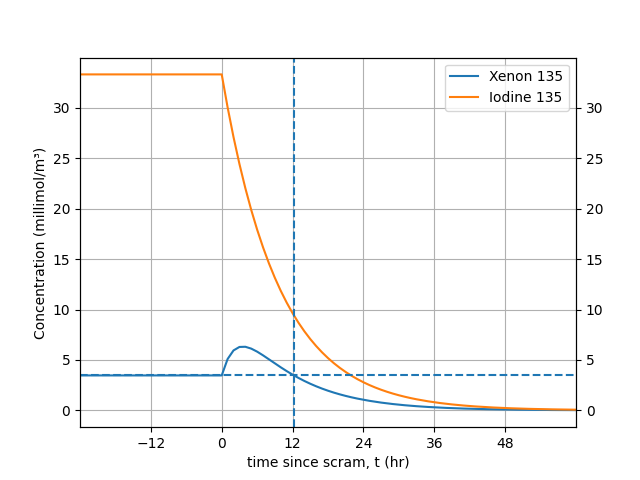
\includegraphics[width=0.99\textwidth]{../img/12hr_restart}
                \caption{Nuclide Concentration - 12-hr Restart}
            \end{figure}
            }
            \only<3-4>{
                \begin{figure}
                %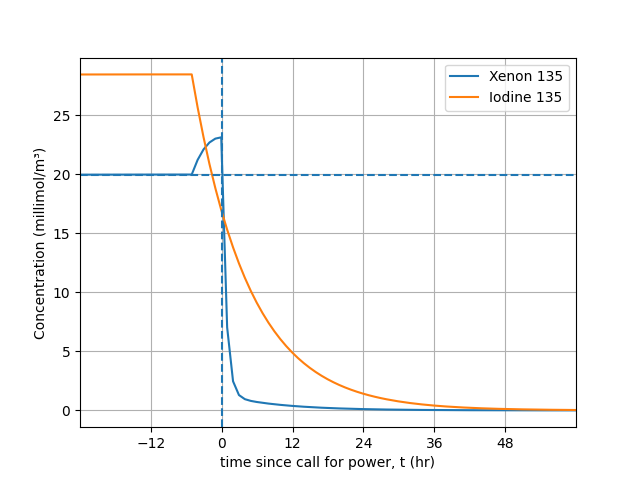
\includegraphics[width=0.99\textwidth]{../img/standby_restart.png}
                \caption{Nuclide Concentration - Standby Restart}
            \end{figure}
            }
        \end{column}
    \end{columns}
\end{frame}

\begin{frame}{Final Remarks}
    
\end{frame}

\begin{frame}{Acknowledgements}
    \centering
    The first author is funded by the Nuclear Regulatory Commission (NRC) in pursuit of an M.S. in Nuclear Engineering.
\end{frame}


\begin{frame}{References}
    \bibliographystyle{neup}
    \footnotesize
    \bibliography{References}
\end{frame}


\end{document}
